Machine learning corresponds to the study and construction of systems that can learn from data. These systems can be useful when typical rule based programs that follow explicit instructions do not give good performance. Their ability to learn makes them popular in the field of artificial intelligence and pattern recognition. Machine learning can take several forms. In this paper, we look specifically at classifiers within the field of supervised learning. In supervised learning the system is trained or `taught' using input data that is known to belong to a certain class of output.\\ 
%A mapping between the inputs and outputs is inferred from the training data which can be used to classify unseen data. \cite{cord2008machine}

For the purpose of understanding how supervised learning works, consider a supervised learning model that is shown in fig \ref{fig:SL}. First step is to normalize raw data and prepare data for the training set and validation set. Next data is randomly allocated to these two sets (usually 60\% for the training set and the rest for validation set). The training set is used by classifier to learn how to classify the data. The training data will feed into the algorithm in order to learn from training data so that it designs a model that wishes to predict an unseen data. When the model is built, validation set analyzes the model by testing its accuracy. It is important in this stage to use data that are not used by the model before, this is why in the second step of figure \ref{fig:SL} the data is split into two.  If a validation set gives out an error rate larger than the training set, then we have to go back, tweak the model and adjust the parameters. Since the build model has already seen the training data, and has memorized the answer, is not trustworthy anymore. As a consequence, the model tries to `memorize' the data instead of `learning' to generalizes. This will make generalization properties of the model, to become progressively worse and is known as over-fitting or over-training\cite{wiki:of} problem in machine learning. However, depending on the type of a classifier, there are techniques to avoid this problem, e.g. to avoid over-fitting in neural network training\cite{Piotrowski201397}. The moment that model shows consistency, it can be used to predict and label an unknown data. \\  
 
\begin{figure}[H]
\centering
    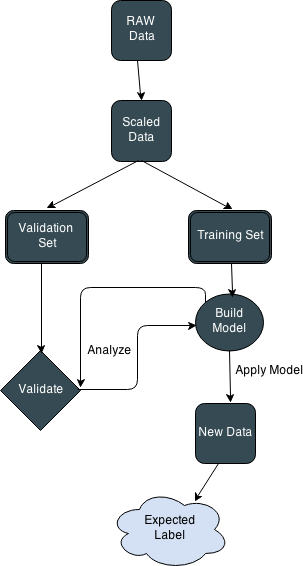
\includegraphics[width=38mm,scale=0.3]{./img/SL.png}
    \caption{\footnotesize{An overview of Supervised learning model that divides scaled data into two sets in order to build a model and predict unseen data }}
    \label{fig:SL}
\end{figure}

In unsupervised learning, no associated label, which is the desired output for a set of inputs, is given to the learning algorithm. The class belonging to each instance in the dataset is unknown and there is no reward when the classifier picks the right class. This technique is therefore more often used when trying to discover hidden classes in new datasets \cite{maglogiannis2007emerging}.






